% This example is meant to be compiled with lualatex or xelatex
% The theme itself also supports pdflatex
\PassOptionsToPackage{unicode}{hyperref}
\documentclass[aspectratio=1610, 12pt, xcolor=dvipsnames]{beamer}

% Warning, if another latex run is needed
% \usepackage[aux]{rerunfilecheck}

% just list chapters and sections in the toc, not subsections or smaller
\setcounter{tocdepth}{1}

%------------------------------------------------------------------------------
%------------------------------ Fonts, Unicode, Language ----------------------
%------------------------------------------------------------------------------
\usepackage{fontspec}
\defaultfontfeatures{Ligatures=TeX}  % -- becomes en-dash etc.

% german language
\usepackage{polyglossia}
\setdefaultlanguage{german}

% for english abstract and english titles in the toc
\setotherlanguages{english}

% intelligent quotation marks, language and nesting sensitive
\usepackage[autostyle]{csquotes}

% microtypographical features, makes the text look nicer on the small scale
\usepackage{microtype}

% colors and stuff
\usepackage{xcolor}
\usepackage[most]{tcolorbox}
\tcbset{on line, hbox,
        boxsep=4pt, left=0pt,right=0pt,top=0pt,bottom=0pt,
        colframe=white,colback=SpringGreen,
        highlight math style={enhanced}
        }
\newtcolorbox{mybox}[3][]
{
  colframe = #2!25,
  colback = #2!20,
  coltitle = #2!20!black,
  title = {#3},
  #1
}
%\colorlet{Green!40}
%------------------------------------------------------------------------------
%------------------------ Math Packages and settings --------------------------
%------------------------------------------------------------------------------

\usepackage{amsmath}
\usepackage{amssymb}
\usepackage{mathtools}
\usepackage{bbold}
\usepackage{hyperref}
\usepackage{url}

% Enable Unicode-Math and follow the ISO-Standards for typesetting math
\usepackage[
  math-style=ISO,
  bold-style=ISO,
  sans-style=italic,
  nabla=upright,
  partial=upright,
]{unicode-math}
\setmathfont{Latin Modern Math}

% nice, small fracs for the text with \sfrac{}{}
\usepackage{xfrac}


%------------------------------------------------------------------------------
%---------------------------- Numbers and Units -------------------------------
%------------------------------------------------------------------------------

\usepackage[
  locale=DE,
  separate-uncertainty=true,
  per-mode=symbol-or-fraction,
]{siunitx}
\sisetup{math-micro=\text{µ},text-micro=µ}
% \sisetup{tophrase={{ to }}}
%------------------------------------------------------------------------------
%-------------------------------- tables  -------------------------------------
%------------------------------------------------------------------------------

\usepackage{booktabs}       % \toprule, \midrule, \bottomrule, etc

%------------------------------------------------------------------------------
%-------------------------------- graphics -------------------------------------
%------------------------------------------------------------------------------

\usepackage{graphicx}
%\usepackage{rotating}
\usepackage{grffile}
\usepackage{tikz}
\usepackage{circuitikz}
\usepackage{tikz-feynman}
\usepackage{subcaption}

% allow figures to be placed in the running text by default:
\usepackage{scrhack}
\usepackage{float}
\floatplacement{figure}{htbp}
\floatplacement{table}{htbp}

% keep figures and tables in the section
\usepackage[section, below]{placeins}

% smileys
\usepackage{MnSymbol,wasysym}

%------------------------------------------------------------------------------
%---------------------- customize list environments ---------------------------
%------------------------------------------------------------------------------

\usepackage{enumitem}
\usepackage{listings}
\usepackage{hepunits}

\usepackage{pdfpages}
%------------------------------------------------------------------------------
%------------------------------ Bibliographie ---------------------------------
%------------------------------------------------------------------------------

\usepackage[
  backend=biber,   % use modern biber backend
  autolang=hyphen, % load hyphenation rules for if language of bibentry is not
                   % german, has to be loaded with \setotherlanguages
                   % in the references.bib use langid={en} for english sources
]{biblatex}
\addbibresource{references.bib}  % the bib file to use
\DefineBibliographyStrings{german}{andothers = {{et\,al\adddot}}}  % replace u.a. with et al.


% Load packages you need here
% \usepackage{polyglossia}
% \setmainlanguage{german}

\usepackage{csquotes}


% \usepackage{amsmath}
% \usepackage{amssymb}
% \usepackage{mathtools}

\usepackage{bookmark}

% load the theme after all packages

\usetheme[
  showtotalframes, % show total number of frames in the footline
]{tudo}

% Put settings here, like
\unimathsetup{
  math-style=ISO,
  bold-style=ISO,
  nabla=upright,
  partial=upright,
  mathrm=sym,
}

% \setbeamertemplate{itemize item}{\scriptsize$\blacktriangleright$}
% \setbeamertemplate{itemize subitem}{\scriptsize$\blacktriangleright$}

%Titel:
\title{Performance of the SciFi Tracker alignment in 2024}
%Autor
\author[N.Breer]{\textbf{Nils Breer}, Biljana Mitreska, Johannes Albrecht}
%Lehrstuhl/Fakultät
\institute{DPG Conference 2025, Göttingen}
%Titelgrafik muss ich einfueren!!!
%\titlegraphic{\includegraphics[width=0.3\textwidth]{content/Bilder/interferenz.jpg}}
\date{02.04.2025}

\begin{document}
\maketitle

\begin{frame}\frametitle{Why do we need detector alignment?}
  \begin{columns}
    \begin{column}[c]{0.5\textwidth}
      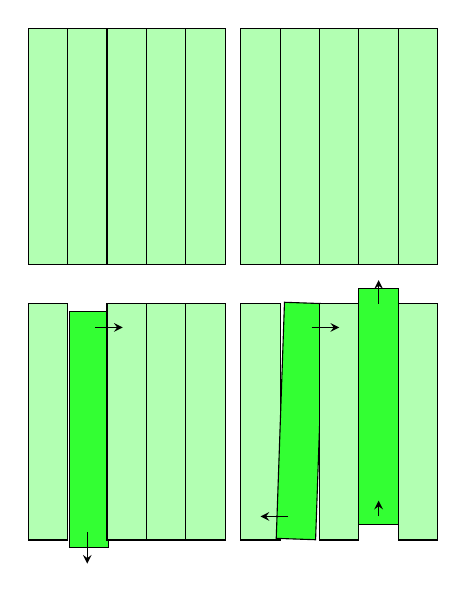
\begin{tikzpicture}
  % this is the ideal detector
  \node[rectangle,
      draw = black,
      % text = ,
      fill = green!30!white,
      minimum width = 0.5cm,
      minimum height = 3cm] (r) at (0,0) {};
  \node[rectangle,
      draw = black,
      % text = ,
      fill = green!80!white,
      minimum width = 0.5cm,
      minimum height = 3cm] (r) at (0.525,-0.1) {};
  \node[rectangle,
      draw = black,
      % text = ,
      fill = green!30!white,
      minimum width = 0.5cm,
      minimum height = 3cm] (r) at (1,0) {};
  \node[rectangle,
      draw = black,
      % text = ,
      fill = green!30!white,
      minimum width = 0.5cm,
      minimum height = 3cm] (r) at (1.5,0) {};
  \node[rectangle,
      draw = black,
      % text = ,
      fill = green!30!white,
      minimum width = 0.5cm,
      minimum height = 3cm] (r) at (2,0) {};

  \node[rectangle,
      draw = black,
      % text = ,
      fill = green!30!white,
      minimum width = 0.5cm,
      minimum height = 3cm] (r) at (2.7,0) {};
  \node[rectangle,
      draw = black,
      % text = ,
      fill = green!80!white,
      rotate around = {-2:(3.2,0)},
      minimum width = 0.5cm,
      minimum height = 3cm] (r) at (3.2,-0.1) {};
  % \draw (2.7,0) -- (5.7,0);
  \node[rectangle,
      draw = black,
      % text = ,
      fill = green!30!white,
      minimum width = 0.5cm,
      minimum height = 3cm] (r) at (3.7,0) {};
  \node[rectangle,
      draw = black,
      % text = ,
      fill = green!80!white,
      minimum width = 0.5cm,
      minimum height = 3cm] (r) at (4.2,0.2) {};
  \node[rectangle,
      draw = black,
      % text = ,
      fill = green!30!white,
      minimum width = 0.5cm,
      minimum height = 3cm] (r) at (4.7,0) {};

% now below it the physical detector
\node[rectangle,
    draw = black,
    % text = ,
    fill = green!30!white,
    minimum width = 0.5cm,
    minimum height = 3cm] (r) at (0,3.5) {};
\node[rectangle,
    draw = black,
    % text = ,
    fill = green!30!white,
    minimum width = 0.5cm,
    minimum height = 3cm] (r) at (0.5,3.5) {};
\node[rectangle,
    draw = black,
    % text = ,
    fill = green!30!white,
    minimum width = 0.5cm,
    minimum height = 3cm] (r) at (1,3.5) {};
\node[rectangle,
    draw = black,
    % text = ,
    fill = green!30!white,
    minimum width = 0.5cm,
    minimum height = 3cm] (r) at (1.5,3.5) {};
\node[rectangle,
    draw = black,
    % text = ,
    fill = green!30!white,
    minimum width = 0.5cm,
    minimum height = 3cm] (r) at (2,3.5) {};

\node[rectangle,
    draw = black,
    % text = ,
    fill = green!30!white,
    minimum width = 0.5cm,
    minimum height = 3cm] (r) at (2.7,3.5) {};
\node[rectangle,
    draw = black,
    % text = ,
    fill = green!30!white,
    minimum width = 0.5cm,
    minimum height = 3cm] (r) at (3.2,3.5) {};
\node[rectangle,
    draw = black,
    % text = ,
    fill = green!30!white,
    minimum width = 0.5cm,
    minimum height = 3cm] (r) at (3.7,3.5) {};
\node[rectangle,
    draw = black,
    % text = ,
    fill = green!30!white,
    minimum width = 0.5cm,
    minimum height = 3cm] (r) at (4.2,3.5) {};
\node[rectangle,
    draw = black,
    % text = ,
    fill = green!30!white,
    minimum width = 0.5cm,
    minimum height = 3cm] (r) at (4.7,3.5) {};

% draw arrows indicating the movement
% x and y translation
\draw [-stealth] (0.6,1.2) -- (0.95,1.2);
\draw [-stealth] (0.5,-1.4) -- (0.5,-1.8);

% rotation
\draw [-stealth] (3.35,1.2) -- (3.7,1.2);
\draw [-stealth] (3.05,-1.2) -- (2.7,-1.2);
% single translation
\draw [-stealth] (4.2,1.5) -- (4.2,1.8);
\draw [-stealth] (4.2,-1.2) -- (4.2,-1);

\end{tikzpicture}

    \end{column}
    \begin{column}[c]{0.5\textwidth}
      \begin{itemize}
        \item $\bullet$\, Track reconstruction: detector position in reconstruction similar to real detector
        \item $\bullet$\, Top: ideal detector, bottom: physical detector
        \item $\bullet$\, Surveys: find the rotation and position of each detector component
        \item $\bullet$\, Surveyed measurements of detector: Input for alignment
        \item $\bullet$\, Alignment goal: achieve the best precision in the detector position
      \end{itemize}
    \end{column}
  \end{columns}
\end{frame}

\begin{frame}\frametitle{Importance of alignments}
  \begin{itemize}
    \item $\bullet$\, Alignment is part of the LHCb trigger system
    \item $\bullet$\, Physics performance tied to alignment performance
    \item $\bullet$\, Good quality alignment contributes to:
    \begin{itemize}
      \item $\bullet$\, \to\, remove systematic biases for asymmetry measurements
      \item $\bullet$\, Best possible mass resolution
    \end{itemize}
  \end{itemize}
  % note: say in the talk: the alignment takes input from events selected by HLT1 to perform the calibration. the updated geometry constants are then applied both to HLT1 and HLT2
  \begin{figure}
      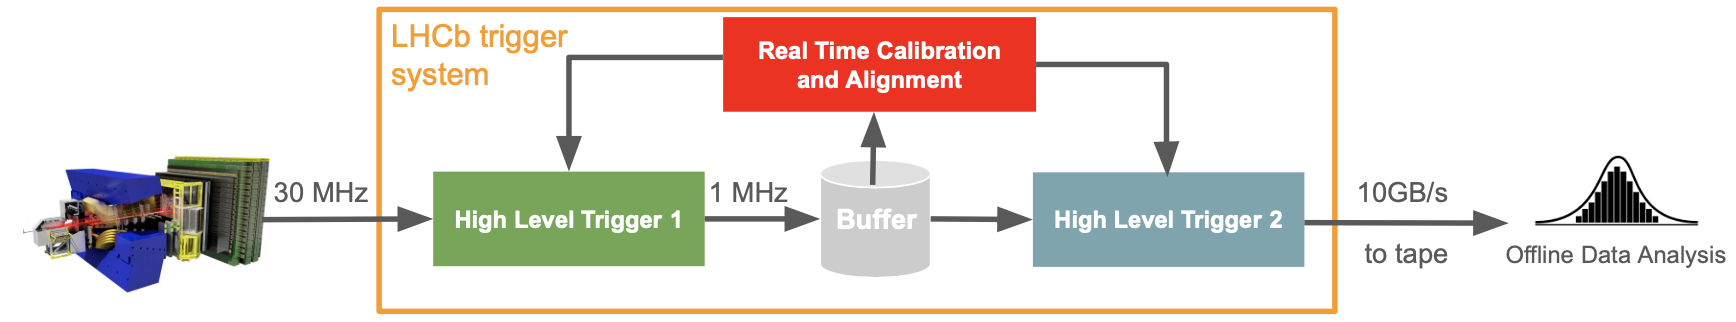
\includegraphics[width=0.9\textwidth]{logos/dataflow.png}%
    % \caption{Hits on tracks in x-direction with run 256145 data on 20000 ents using 9 minimum hits against 11 minimum hits.}
  \end{figure}
\end{frame}

\begin{frame}\frametitle{Tracking alignment: track fit using Kalman filter}
  \begin{itemize}
    \item $\bullet$\, Input sample: reconstructed tracks (HLT2)
    \item $\bullet$\, $\chi^2$ minimization algorithm \to\, determine detector element position
  \end{itemize}
  \begin{figure}
    \centering
    % 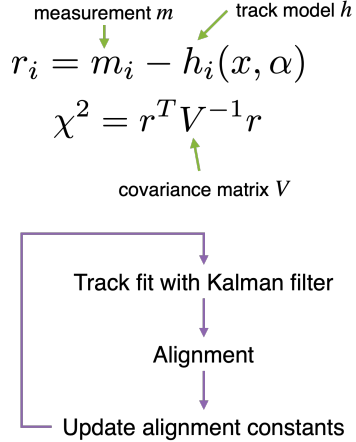
\includegraphics[width=0.72\textwidth]{logos/kalman.png}
    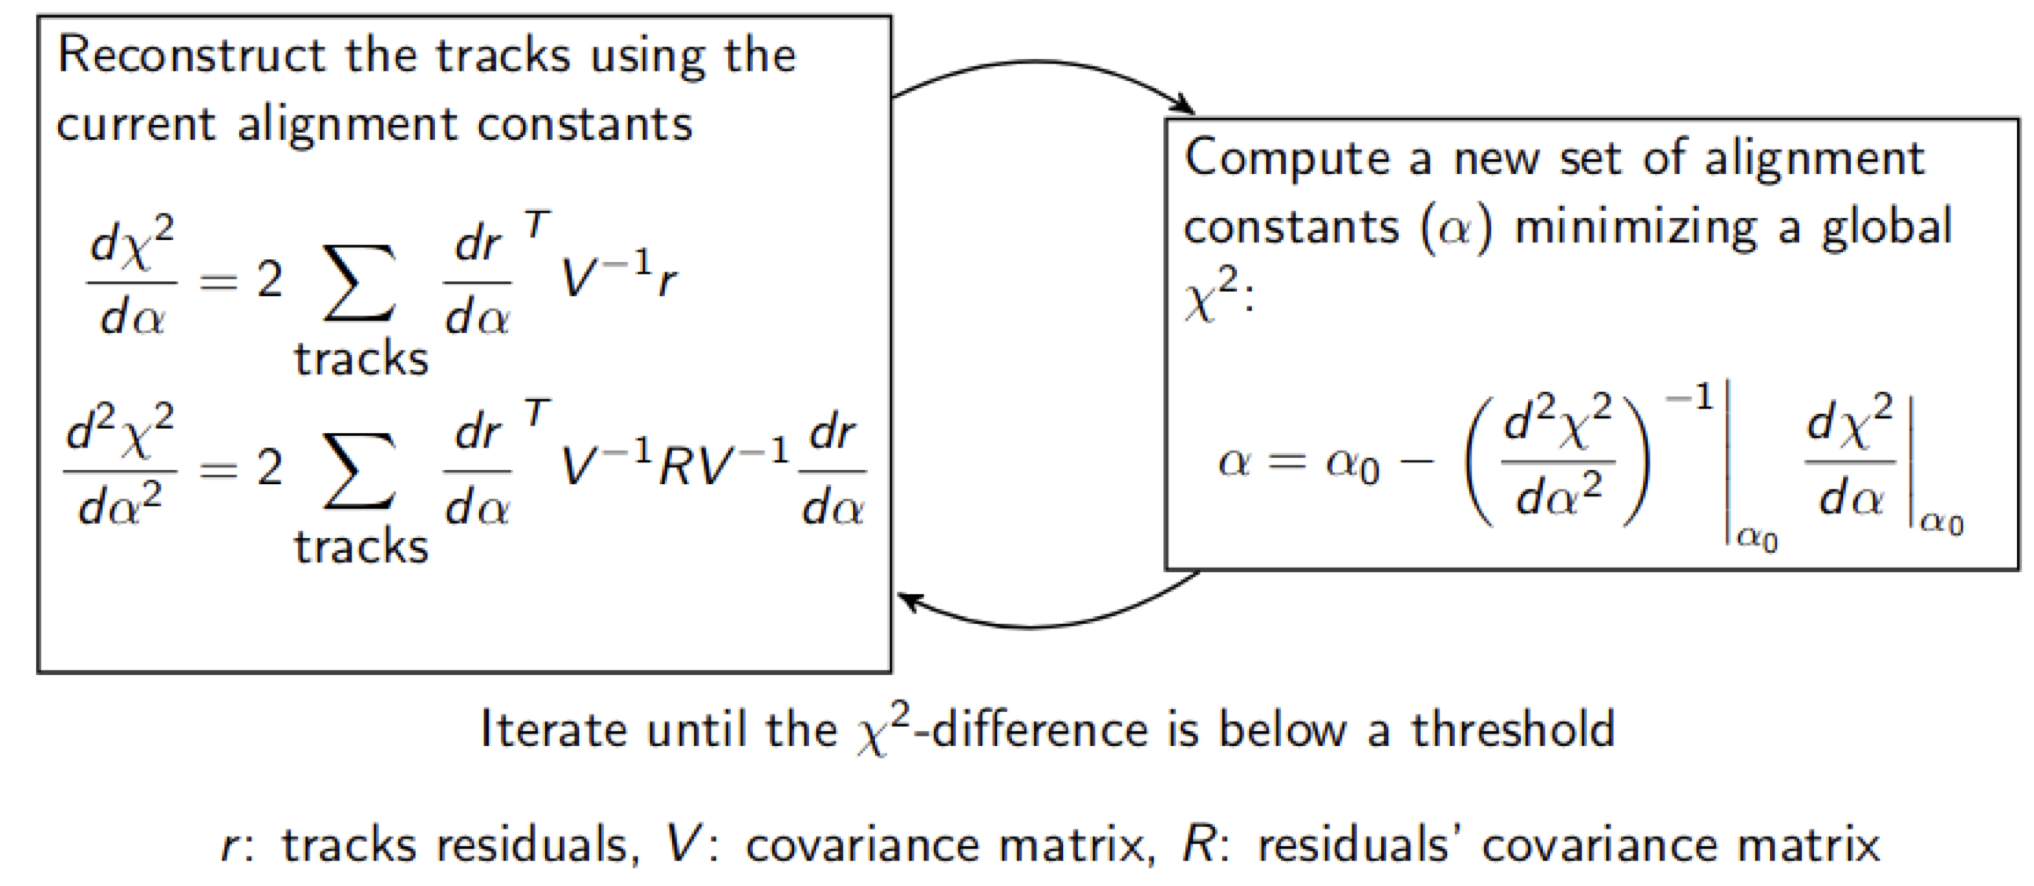
\includegraphics[width=0.7\textwidth]{plots/kalman_real.png}
  \end{figure}
  \begin{itemize}
    % \item $\bullet$\, Add measurements one-by-one to fit
    % \item $\bullet$\, Prediction of next measurement \to minimize residuals \to redo until track complete
    \item $\bullet$\, Easily models material interactions as well as multiple scattering
  \end{itemize}
\end{frame}

\begin{frame}\frametitle{The Run 3 LHCb detector}
  \begin{columns}
    \begin{column}[c]{0.6\textwidth}
      \begin{figure}
        % 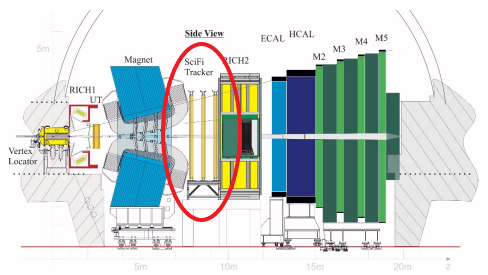
\includegraphics[width=\textwidth]{logos/upgrade_lhcb.png}
        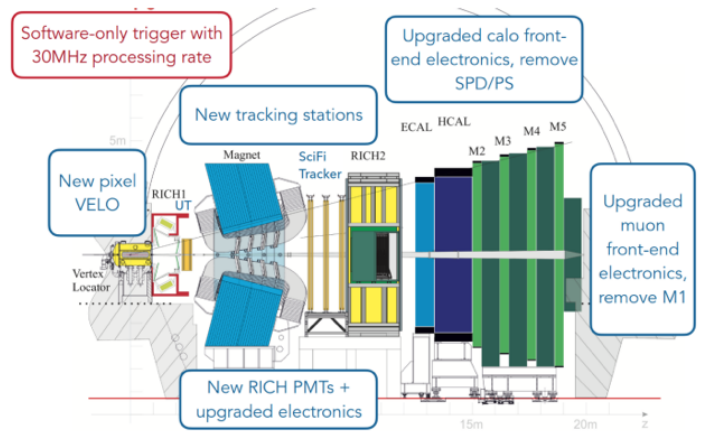
\includegraphics[width=\textwidth]{plots/lhcb_upgrade.png}
        % \caption{Visualization of the SciFi tracking stations.}
      \end{figure}
    \end{column}
    \begin{column}{0.48\textwidth}
      \begin{itemize}
        \item $\bullet$\, Brand new detector to maintain physics performance at more radiation harsh environment
        \item $\bullet$\, UT was not present during 2022-23 data taking \to focus on SciFi and VELO
      \end{itemize}
      \begin{figure}
        \centering
        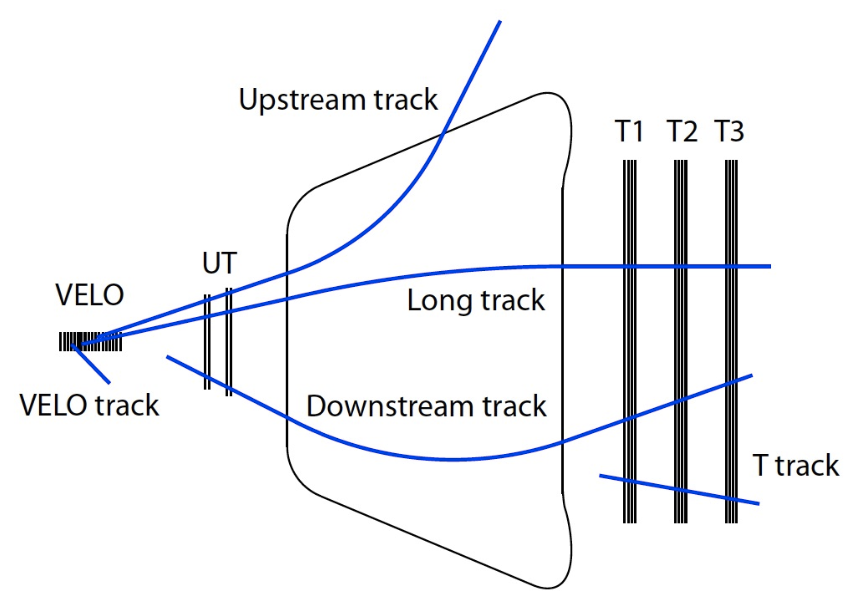
\includegraphics[width=0.8\textwidth]{track.png}
      \end{figure}
    \end{column}
  \end{columns}
\end{frame}

\begin{frame}\frametitle{The Scintillating Fibre Tracker}
  \begin{columns}
    \begin{column}[c]{0.48\textwidth}
      \begin{figure}
        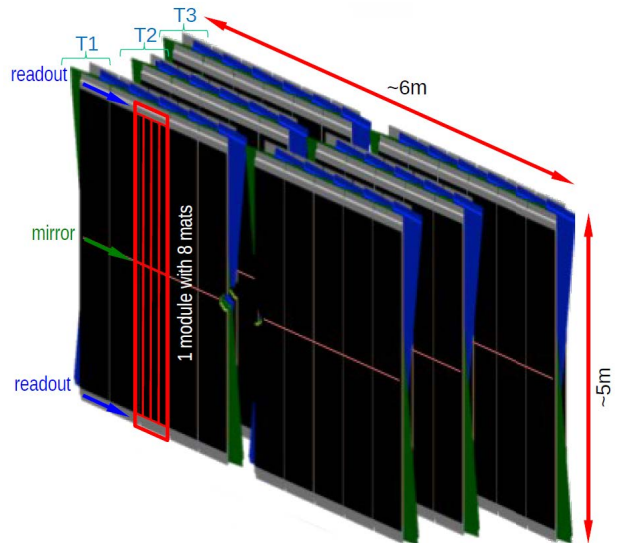
\includegraphics[width=0.9\textwidth]{logos/scifi.png}
        % \caption{Visualization of the SciFi tracking stations.}
      \end{figure}
    \end{column}
    \begin{column}{0.48\textwidth}
      \begin{itemize}
        \item $\bullet$\, 5 modules per side except for back T-station has 6
        \item $\bullet$\, X1, X2-layers are vertical and only yield x-position information
        \item $\bullet$\, U, V layers have a $\mp 5 \si{degree}$ stereo angle respectively
        \begin{itemize}
          \item $\bullet$\, \to\, Used for determining y-position of tracks by comparing hitposition at different angles
        \end{itemize}
      \end{itemize}
    \end{column}
  \end{columns}
\end{frame}

\begin{frame}\frametitle{VELO geometry}
  \begin{columns}
    \begin{column}[c]{0.5\textwidth}
      \begin{itemize}
        \item $\bullet$\, Rotation Rz leading to shifts in x and y
        % \item half alignment somewhat sensitive and shows Rz ≈ 3 mrad
        \item $\bullet$\, Half alignment sensitive to x shift
        \item $\bullet$\, Global movement in y
        \begin{itemize}
          \item $\bullet$\, Can not be corrected for by half alignment
        \end{itemize}
      \end{itemize}    
    \end{column}
    \begin{column}[c]{0.5\textwidth}
      \begin{figure}
        \centering
        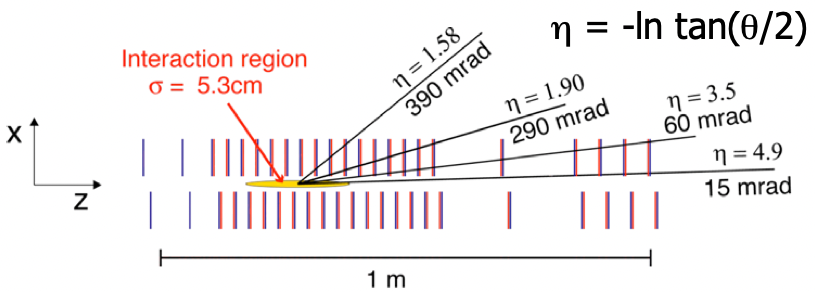
\includegraphics[width=\textwidth]{plots/velo_layers_all.png}
      \end{figure}
    \end{column}
  \end{columns}
  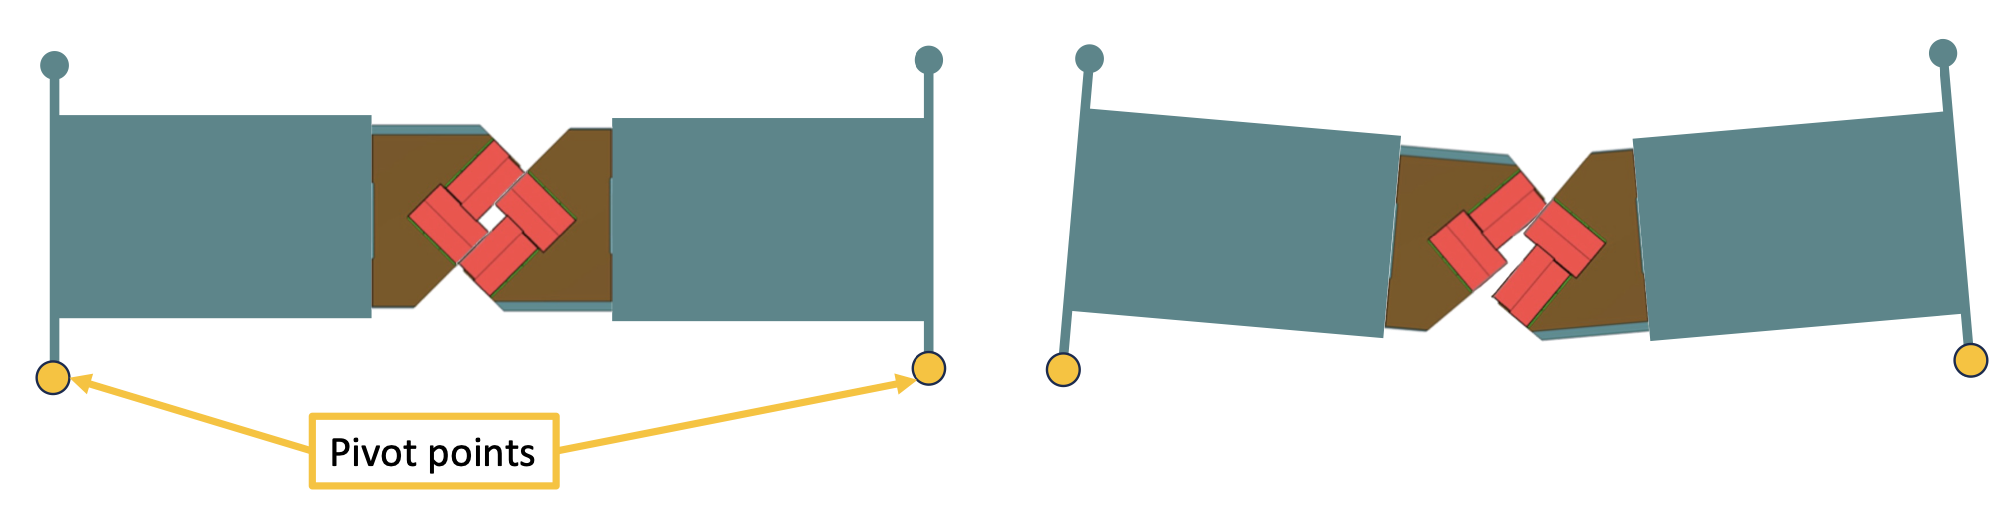
\includegraphics[width=\textwidth]{plots/velo_rotation.png}
\end{frame}

\begin{frame}\frametitle{Global alignment and motivation for precision studies}
  \begin{mybox}{green}{Global alignment}
    \begin{itemize}
      \item $\bullet$\, Alignment of the VELO, SciFi and UT simultaneously
    \end{itemize}
    \begin{itemize}
      \setlength\itemsep{0em}
      \item $\bullet$\, Motivation for global alignment
      \begin{itemize}
        \item $\bullet$\, Understanding the interplay between tracking systems
        \item $\bullet$\, Rotations inside the VELO \to weak modes inside SciFi (VELO twisting)
      \end{itemize}
    \end{itemize}
  \end{mybox}
  \begin{mybox}{yellow}{Precision studies}
    \begin{itemize}
      \item $\bullet$\, Analyzing the precision of the SciFi tracker on 2024 data
      \begin{itemize}
        \setlength\itemsep{0em}
        \item $\bullet$\, Obtain precision by running over a set of runs throughout the year \to automatic uptdate threshold 
        \item $\bullet$\, Exceeding this threshold triggers an alignment update
      \end{itemize}
    \end{itemize}
  \end{mybox}
\end{frame}

\begin{frame}\frametitle{Detectorposition in 2024}
  \begin{columns}
    \begin{column}[c]{0.48\textwidth}
      \begin{figure}
        \centering
        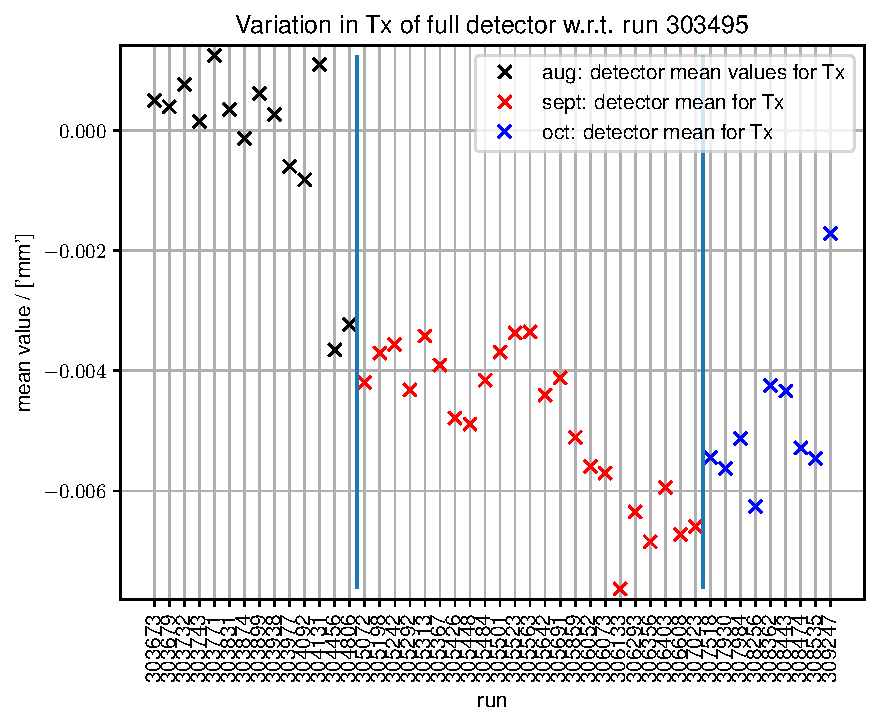
\includegraphics[width=\textwidth]{plots/2025_plots_goettingen/scifi_stability_outdir_18102024/full/stabi_test_Tx_full_normal_variation.pdf}
      \end{figure}
    \end{column}
    \begin{column}[c]{0.48\textwidth}
      \begin{itemize}
        \item $\bullet$\, Aligning SciFi CFrames in Tx and modules in Tx
        \item $\bullet$\, mean module constant for the whole SciFi w.r.t. reference run from 2024 alignment update 
        \item $\bullet$\, distinct edges at points of interest (hardware, machine development)
        \item $\bullet$\, The movements may not always come from the SciFi \to related to the VELO position
      \end{itemize}
    \end{column}
  \end{columns}
\end{frame}

\begin{frame}\frametitle{Detectorposition in 2024, halfmodules Rx alignment}
  \begin{columns}
    \begin{column}[c]{0.48\textwidth}
      \begin{figure}
        \centering
        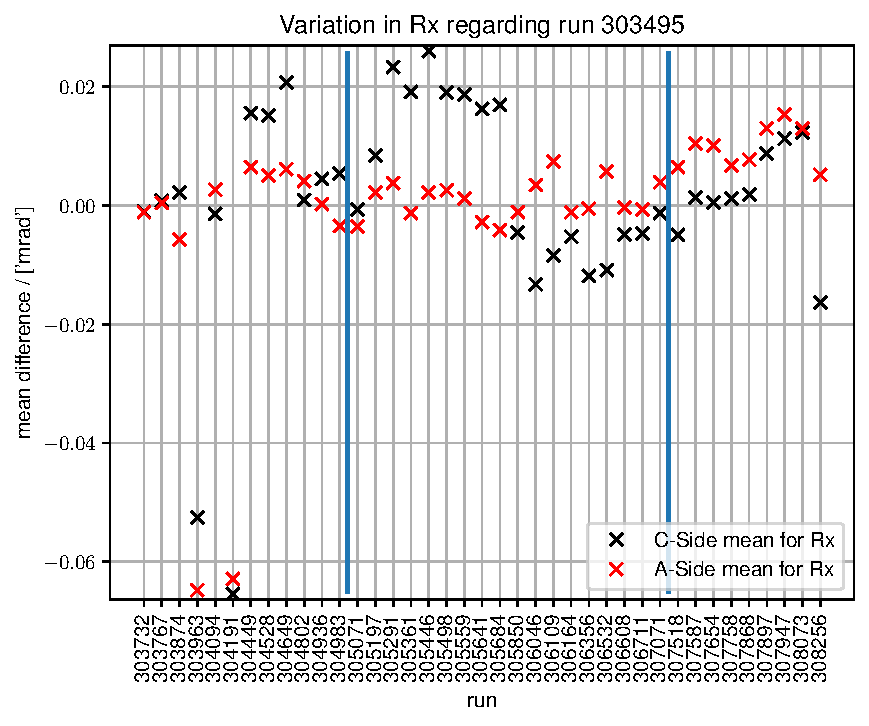
\includegraphics[width=\textwidth]{plots/2025_plots_goettingen/scifi_stability_halfmodules_outdir_jan2025/half/stabi_test_Rx_half.pdf}
      \end{figure}
    \end{column}
    \begin{column}[c]{0.48\textwidth}
      \begin{itemize}
        \item $\bullet$\, Rerunning the test with halfmodule alignment in Rx (here) as well as TxRz and CFrames in Tx
        \item $\bullet$\, Fluctuation is seen in the SciFi C side
        \begin{itemize}
          \item $\bullet$\, VELO constants follow the same trend until "edges" seen in the constants \to not the cause for this effect
          \item $\bullet$\, Related to the alignment of the VELO halves
        \end{itemize}
      \end{itemize}
    \end{column}
  \end{columns}
\end{frame}

\begin{frame}\frametitle{Detectorposition in 2024, halfmodules TxRz alignment}
  \begin{itemize}
    \setlength\itemsep{0em}
    \item $\bullet$\, Halfmodules aligned in TxRz and CFrames in Tx
    \item $\bullet$\, Per layer, movement looks consistent over all runs \to expected
  \end{itemize}
  \begin{columns}
    \begin{column}[c]{0.5\textwidth}
      \begin{figure}
        \centering
        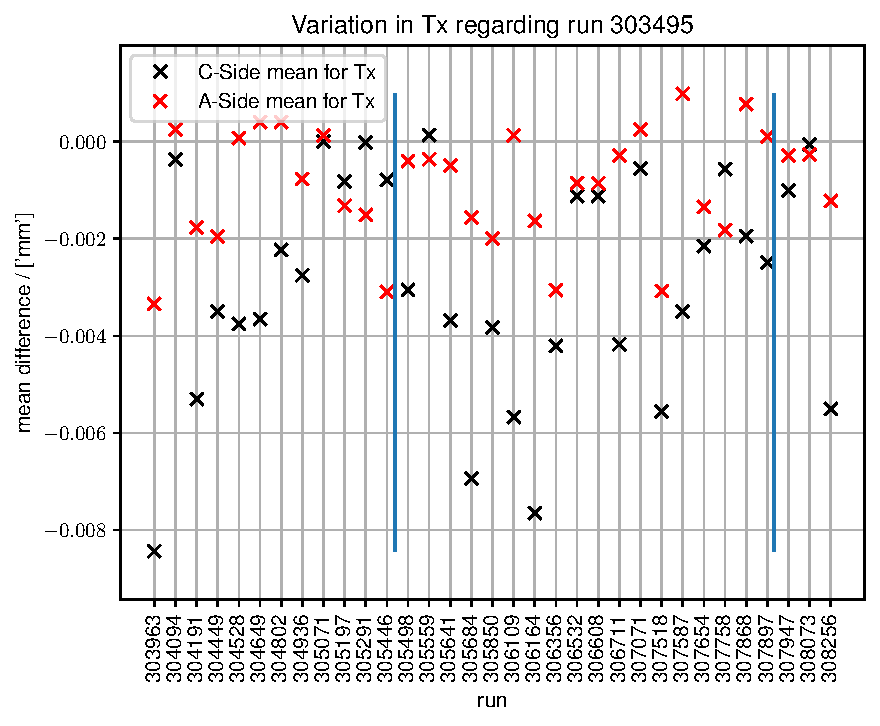
\includegraphics[width=0.8\textwidth]{plots/2025_plots_goettingen/scifi_stability_TxRz/half/stabi_test_Tx_half_correct.pdf}
      \end{figure}
    \end{column}
    \begin{column}[c]{0.5\textwidth}
      \begin{figure}
        \centering
        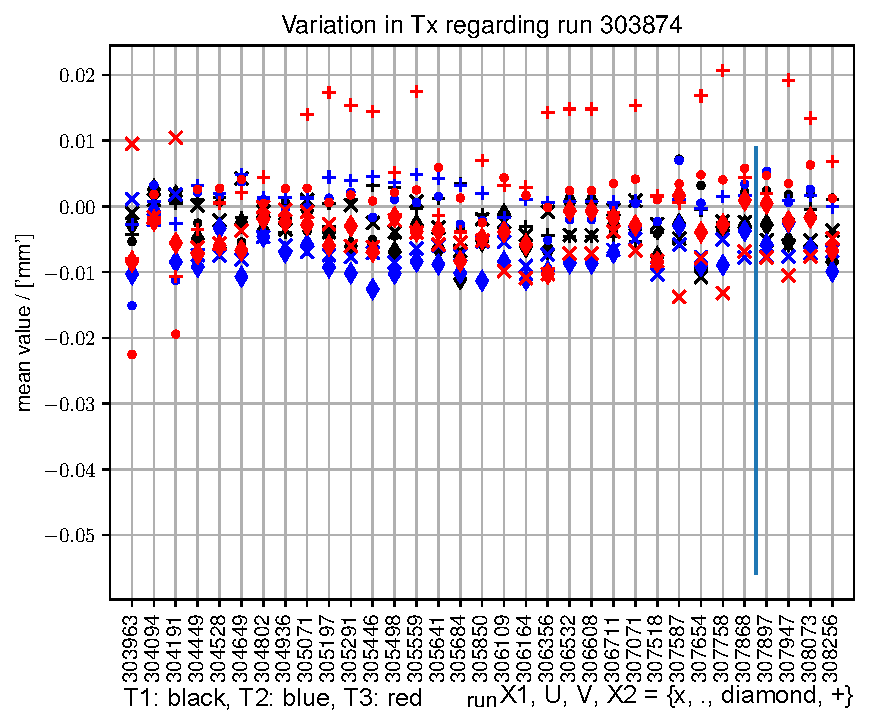
\includegraphics[width=0.8\textwidth]{plots/2025_plots_goettingen/scifi_stability_TxRz/per_layer/stabi_test_Tx_per_layer.pdf}
      \end{figure}
    \end{column}
  \end{columns}
\end{frame}

\begin{frame}\frametitle{Detectorposition in 2024}
  \begin{itemize}
    \setlength\itemsep{0em}
    \item $\bullet$\, Width of the distribution is a wider in the last station \to also seen on Monte Carlo
    \item $\bullet$\, Overall centered and width is comparable to MC values
  \end{itemize}
  \begin{columns}
    \begin{column}[c]{0.5\textwidth}
      \begin{figure}
        \centering
        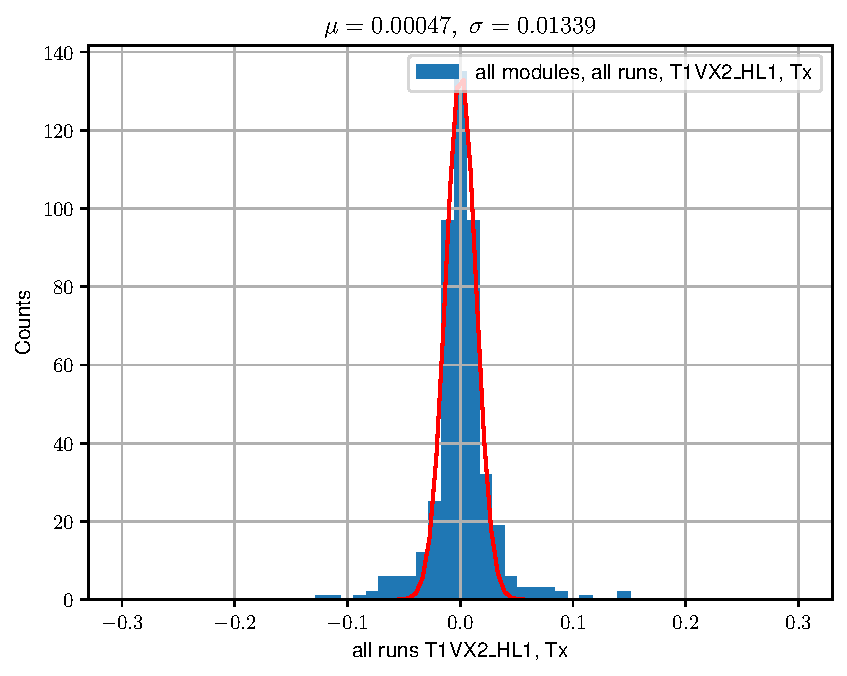
\includegraphics[width=0.8\textwidth]{plots/2025_plots_goettingen/scifi_stability_TxRz/module_per_cframe/stabi_test_Tx_module_per_cframe_all_modules_T1VX2_HL1.pdf}
      \end{figure}
    \end{column}
    \begin{column}[c]{0.5\textwidth}
      \begin{figure}
        \centering
        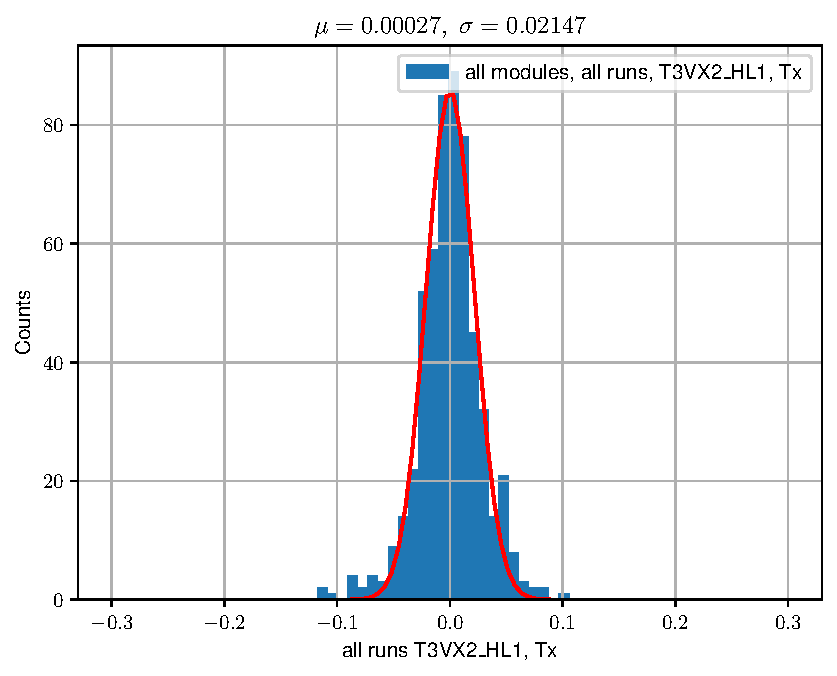
\includegraphics[width=0.8\textwidth]{plots/2025_plots_goettingen/scifi_stability_TxRz/module_per_cframe/stabi_test_Tx_module_per_cframe_all_modules_T3VX2_HL1.pdf}
      \end{figure}
    \end{column}
  \end{columns}
\end{frame}

\begin{frame}\frametitle{Summary}
  \begin{itemize}
    \setlength\itemsep{0em}
    \item $\bullet$\, The precision study for the 2024 data since the v21 alignment update looks consistent and shows expected behavior \to data taken in 2024 is good!
    \item $\bullet$\, Better than the single hit resolution of the SciFi of $\SI{100}{\micro\metre}$
    \item $\bullet$\, Comparison to Monte Carlo is consistent
    \item $\bullet$\, Still need to understand the difference seen between spread in SciFi stations
    \item $\bullet$\, \textbf{Thank you for your attention!}
  \end{itemize}
  % \begin{table}
  %   \begin{tabular}{c c c c}
  %     \toprule
  %      & Modules Tx & Modules Rz \\
  %     \midrule
  %      2024 Data   & \num{13} - \SI{22}{\micro\metre} & \num{10} - \SI{16}{\micro\radian} \\
  %      Monte Carlo & \num{15} - \SI{35}{\micro\metre} & \num{10} - \SI{20}{\micro\radian} \\
  %      % \num{2} - \SI{40}{\micro\metre} & 
  %     \bottomrule
  %   \end{tabular}
  % \end{table}
\end{frame}

\begin{frame}\frametitle{The survey: what is it and the different types}
  \begin{columns}
    \begin{column}[c]{0.48\textwidth}
      $\bullet$\, Measure distance of some points on the detector with a laser
      \begin{figure}
        \centering
        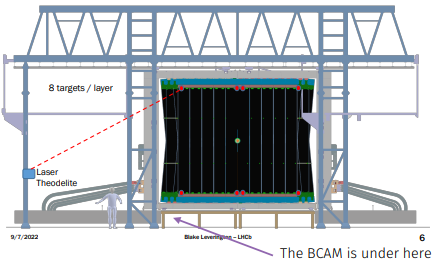
\includegraphics[width=\textwidth]{logos/survey.png}
      \end{figure}
    \end{column}
    \begin{column}[c]{0.48\textwidth}
      \begin{itemize}
        \item $\bullet$\, Layer survey: find corners of layers
        \item $\bullet$\, Module survey: reflective stickers, calculate module plane
        \item $\bullet$\, Compare survey to simulation
      \end{itemize}
    \end{column}
  \end{columns}
\end{frame}

\begin{frame}\frametitle{Alignables for the global alignment}
  \begin{columns}
    \begin{column}[c]{0.5\textwidth}
      \begin{figure}
        \centering
        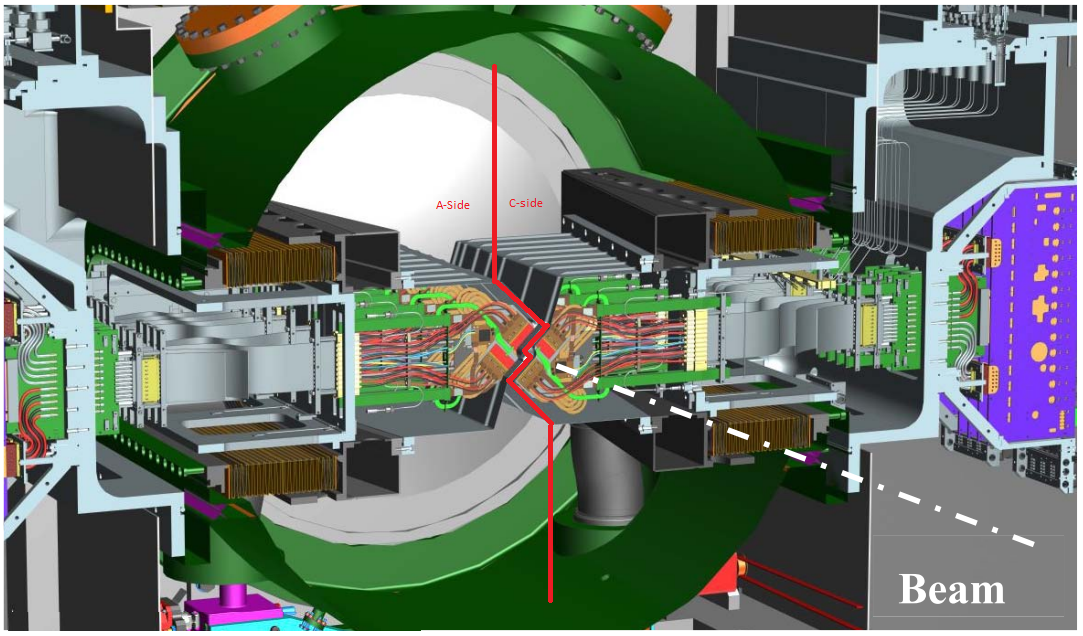
\includegraphics[width=0.9\textwidth]{plots/velo_halves.png}
      \end{figure}
    \end{column}
    \begin{column}{0.5\textwidth}
      \begin{figure}
        \centering
        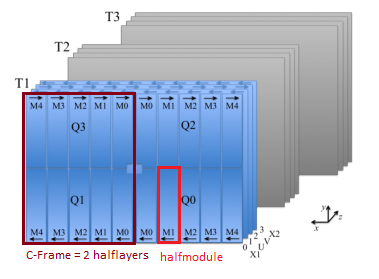
\includegraphics[width=0.9\textwidth]{plots/scifi_modell.png}
      \end{figure}
    \end{column}
  \end{columns}
\end{frame}

% \begin{frame}\frametitle{M5 studies}
%   \begin{columns}
%     \begin{column}[c]{0.5\textwidth}
%       \begin{figure}
%         \centering
%         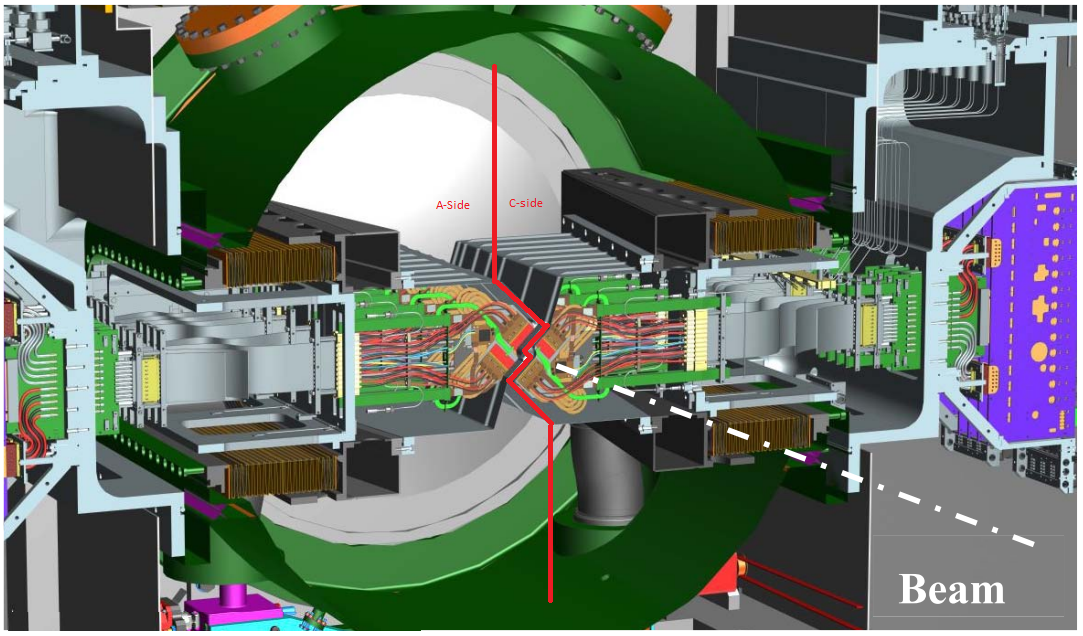
\includegraphics[width=0.9\textwidth]{plots/velo_halves.png}
%       \end{figure}
%     \end{column}
%     \begin{column}{0.5\textwidth}
%       \begin{itemize}
%         \item $\bullet$\, During alignment the M5 modules appear to see little to no hits
%       \end{itemize}
%     \end{column}
%   \end{columns}
% \end{frame}

% \begin{frame}\frametitle{Links}
%   \begin{itemize}
%     \item \href{https://www.sciencedirect.com/science/article/pii/S0168900208017567?ref=pdf_download&fr=RR-2&rr=85f05f5ef91a1973}{Wouter's paper on the Kalman Filter}
%     \item \href{https://indico.bnl.gov/event/19560/contributions/83349/attachments/51225/87618/AI4EIC_2023_Mitreska.pdf}{Real time Alignment and calibration presentation}
%   \end{itemize}
% \end{frame}

\end{document}
